\documentclass[10pt, a4paper]{article}
\usepackage[T2A]{fontenc}
\usepackage[english, russian]{babel}

\usepackage{graphicx}
\graphicspath{{./figs/}}

\usepackage{amsmath}
\usepackage{amssymb}
\usepackage{mathtools}
\usepackage{physics}
\usepackage{upgreek}
\usepackage{sectsty}
\usepackage{color,soul}
\usepackage[colorlinks=true,allcolors=blue]{hyperref}
\sectionfont{\centering}

\usepackage{geometry}
 \geometry{
 a4paper,
 margin=25mm,
 }

\title{Билеты к кандидатскому экзамену по физике плазмы}
\date{}

\begin{document}

\newpage
\section{Термодинамика плазмы}
\label{sec.1}

\subsection{Понятие плазмы, квазинейтральность, микрополя, дебаевский радиус, идеальная и неидеальная плазма.}
\label{sec.1.1}

Плазма~\cite{kotelnikov}. Ссылка на уравнение~\eqref{eq.Euler}, Рис.~\ref{fig.1.2.1}.

\begin{equation}
    \label{eq.Euler}
    e^{i \pi} + 1 = 0
\end{equation}

\subsection{Условие термодинамического равновесия, термическая ионизация, формула Саха, корональное равновесие, снижение потенциала ионизации.}
\label{sec.1.2}

Картинка

\begin{figure}[h!]
    \center{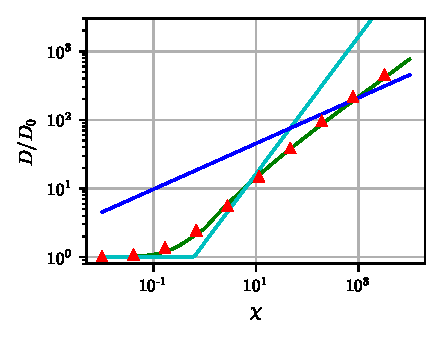
\includegraphics[width=85mm]{test.pdf}}
    \caption{\label{fig.1.2.1} Подпись.}
\end{figure}

\subsection{Вырождение плазмы, статистика Больцмана и Ферми—Дирака, модель Томаса—Ферми.}


\section{Элементарные процессы}
\label{sec.2}

\subsection{Столкновения заряженных частиц, дальнодействие.}
\label{sec.2.1}

[Ю.П. Райзер, Физика Газового разряда, 3-е изд, стр. 29]

Из всех сил взаимодействия между атомными частицами медленнее вceгo спадают с расстоянием (как $1/r^{2}$)  кулоновские силы. Они обладают наибольшим дальнодействием.
За время пролёта t мимо иона, электрон отклоняется на угол $\theta$ . Его можно оценить как отношение полученной поперечной скорости к изначальной скорости:

Основную роль в рассеянии играют столкновения с большим прицельным параметром $\rho$ (рассеяние на малые углы),реализуются при  $\rho > r_{0}$- Кулоновского радиуса (радиус при котором кин. энергия электрона равна потенциальной $ mv^{2}/2 = e^{2}/ r_{0} $,$ r_{0}=e^{2}/mv^{2} $). С другой стороны, потенциал иона спадает $\sim exp(-r/d)/r $. То есть основной вклад вносят столкновения с прицельным параметром от  $r_{0}$   до $d$ (радиус дебая).
Поэтому полное сечение для кулоновских рассеяний $\sigma= \pi*r_{0}^{2} \int_{r_{0}}^{d} r_{0} d\rho/\rho =\pi*r_{0}^{2}*ln{d/r_{0}}$

$ln{d/r_{0}}$ - Кулоновский логарифм.

Столкновения атомных частиц могут иметь упругий и неупругий характер. При упругом соударении меняются направления движения партнеров, происходит обмен импульсом и кинетической энергией, но внутренние энергии и состояния частиц остаются неизменными.

\subsection{Частоты столкновений}
\label{sec.2.2}

[Ю.П. Райзер, Физика Газового разряда, 3-е изд, стр.20]

Число соударений определенного рода, которые данная частица (назовем: ее 1) в среднем совершает в 1 с, двигаясь в газе из частиц мишеней 2, называют частотой столкновений.

$\nu_{1}=N_{2}*v'*\sigma (v')$
, где $v'$ скорость сближения

Для газовой кинетики это тоже работает и если распределение частиц массы М по абсолютным скоростям описывается максвелловской функцией, то вместо скорости надо ставить среднее её значение $\bar{v'}=\sqrt{2} \bar{v}$ ; $\bar{v}=\sqrt{\frac{8kT}{\pi M}}$, где за массу надо брать приведённое её значение по 2-м частицам ($ M=\frac{M_{1} M_{2}}{(M_{1}+M_{2})} $), а за сечение рассеяния $\pi d_{mol}^{2} $

\subsection{Столкновения электронов с атомами (упругие и неупругие)}
\label{sec.2.3}


\subsubsection{Упругие}
\label{sec.2.3.1}
[Астапенко В.А.,Лисица В.С., столкновительные процессы в …... стр.30]


Вычисление сечения процесса является сложным кванто-механическим расчетом и зависит от скорости налетающего электрона. Транспортное сечение выражается сложным образом

$\sigma_{tr}=4\pi (L^{2}+\frac{4}{5}\frac{\pi \alpha L}{a_{bor}}\frac{mV}{\hbar}+\frac{\pi^{2}}{6}\frac{\alpha^{2}}{a_{bor}^{2}}(\frac{mV}{\hbar})^{2})$

Здесь $L$ - длина рассеяния электрона на атоме. Первый член - короткодействующие силы. Последний - дальнодействующий потенциал деполяризационный. Промежуточный - интерфериционный от предыдущих двух (проявляются волновые свойства электрона), он может быть отрицательным (при отрицательном L).
Как именно происходит интерференция - см [И. мак-Даниэль, процессы столкновений в ионизированных газах,гл. 4, §4, стр 161] и [гл. 3, §15, пункт Д, “рассеяние  S волны на сферической потенциальной яме”]

\subsubsection{Неупругие}
\label{sec.2.3.2}

Ионизация

[Астапенко В.А.,Лисица В.С., столкновительные процессы в …... стр.37]

Так как после ионизации мы имеем ситуацию, что электрон улетает от иона, то это мы можем рассматривать как упругое рассеяние электрона на ионе, однако в сечение войдут не все электроны, а лишь с энергией выше, чем $E_{ion}$

$\frac{d\sigma^{(R)}}{d\Omega}=(\frac{Ze^{2}}{2mV^{2}sin^{2}(\frac{\theta}{2})})^{2}$

При рассеянии иону передается импулmc $\Delta p=2mVsin(\theta/2)$ и соответственно энергия $\Delta E=4 E sin^{2}(\theta/2)$ , поэтому можно перейти к интегрированию по энергиям.
$\delta \sigma =\frac {\pi e^{2}d\Delta E}{E(\Delta E)^2}$; 
$\sigma_{ion}=\int_{E_{ion}}^{E} d\sigma=\frac{\pi e^4}{E}(\frac{1}{E_{ion}}-\frac{1}{E})=\frac{\pi e^4}{E_{ion}^{2}}\frac{x-1}{x}$
, где $x=E-E_{ion}$ , то есть ионизация имеет пороговый характер

Возбуждение электронным ударом [Астапенко В.А.,Лисица В.С., столкновительные процессы в …... стр.50]

Уравнение рассматриваемого процесса имеет вид $e + A -> A* + e$. Согласно этому принципу атом при взаимодействии с электромагнитным полем ведёт себя как набор осцилляторов, которые ставятся в соответствие паре энергетических уровней $E_i$ , $E_j$ атомного спектра. Собственные частоты этих осцилляторов равны собственной частоте перехода $i -> j$ , $\omega _{i,j}=\frac{(E_j-E_i)}{\hbar}$ , а эффективность их взаимодействия с электромагнитным полем определяется силой осциллятора:
$f_{i,j}=\frac{2m\omega_{ij} {|d_{ij}|}^{2} }{3\hbar e^{2} g_i}$
, где $g_i$ - статистический вес начального состояния. 

При кванто-механическом описании дипольный момент осциллятора перехода $d_{ij}$ представляет собой матричный элемент ооператора электрического дипольного момента между состояниями $|i>$, $|j>$. В случае возбуждения атома $i,j>0$ и $f_{i,j}>0$, для электронного перехода с уменьшением энергии $i,j<0$ и $f_{i,j}<0$. Также может быть $f_{i,j}=0$, тогда такие переходы называются дипольно-(или оптически) запрещенными. Если  $f_{i,j} \ne 0$ оптически-разрешенный переход.
Предполагая поле налетающего электрона в области локализации атома однородным, можно записать следующее уравнение для радиус-вектора осциллятора $rij$:
$r_{ij}''+\gamma_{ij}r_{ij}'+\omega_{ij}^{2}r_{ij}=f_{i,j}\frac{e}{m}E(t,\rho)$, где $\gamma_{ij}$-константа затухания,  $\rho$- прицельный параметр. Записывается скорость затухания в таком осцилляторе и ищется работа, которую совершает поле над осциллятором за всё время столкновения.
Вероятность возбудить атом будет $W_{ij}(\rho)=\frac {A_{ij}(\rho)}{\hbar_{ij}}$, полное сечение  будет $\sigma_{ij}=2\pi \int_{a}^{\inf} W_{ij}(\rho)\rho d\rho$. Тут, как и в кулоновском рассеянии основную роль играют рассеяние на малые углы, то есть с большим прицельным параметром.
$\sigma_{ij}=\pi f_{ij} \frac {e^{2}}{m\Delta E_{ij} } \int_{a}^{\inf} |E(\omega_{ij},\rho)|^{2} \rho d\rho$
Далее - трудные выкладки с методом функции подобия. Самое главное, характер функции сигмы от энергии. Она выглядит схожим образом с зависимостью сечения ионизации. Также имеет пороговый характер, на бесконечности спадает как $ln(E)/E$. Имеет максимум в при $E=3,45*E_{ij}$
Для запрещенных переходов данный расчёт в дипольном приближении невозможен. ибо носит не дипольный характер. Дипольно-запрещённые переходы бывают двух типов: без изменения спина атома (дипольный момент перехода отсутствует из-за невыполнения правил отбора по орбитальному квантовому числу L, переход осуществляется за счёт прямого кулоновского взаимодействия) и переходы с изменением атомного спина (В этом случае возбуждение атома происходит за счет обменного взаимодействия между налетающим и атомным электроном).



Плазма

\newpage
\addcontentsline{toc}{section}{Список литературы}
\bibliographystyle{unsrt}
\bibliography{program}

\end{document}